%!TEX root = ../../dissertation.tex
\chapter{Apo-State Conformational Changes in ABFEP calculations}
\label{ch:apo-state-conformational-changes}
\section{Introduction}

\lipsum[1][1-3]

\subsection{Background}

\lipsum[1][1-3]

\subsection{Dataset and Systems: A2A Deflorian et al}

\lipsum[1][1-3]

\section{Methods}

\lipsum[1][1-3]

\subsection{System setup}

\lipsum[1][1-3]

\subsection{FEP Simulations and Analysis}

\lipsum[1][1-3]

\subsection{Construction of Binding pocket CVs}

\lipsum[1][1-3]

\subsection{REUS Simulations}

\lipsum[1][1-3]

\section{Identifying issues in apo state representation}

\lipsum[1][1-3]

Full ensemble- and time-coloured projections are provided in
Figures~\ref{fig:si-pca-ensembles} and~\ref{fig:si-pca-time}. Comparisons of apo,
alchemical-endpoint, and holo ensembles across datasets are shown in
Figures~\ref{fig:si-pca-other-datasets} and~\ref{fig:si-pca-deflorian-overlap}.

\section{Correcting for Apo state representation issues}

\lipsum[1][1-3]

\begin{figure}[p]
  \centering
  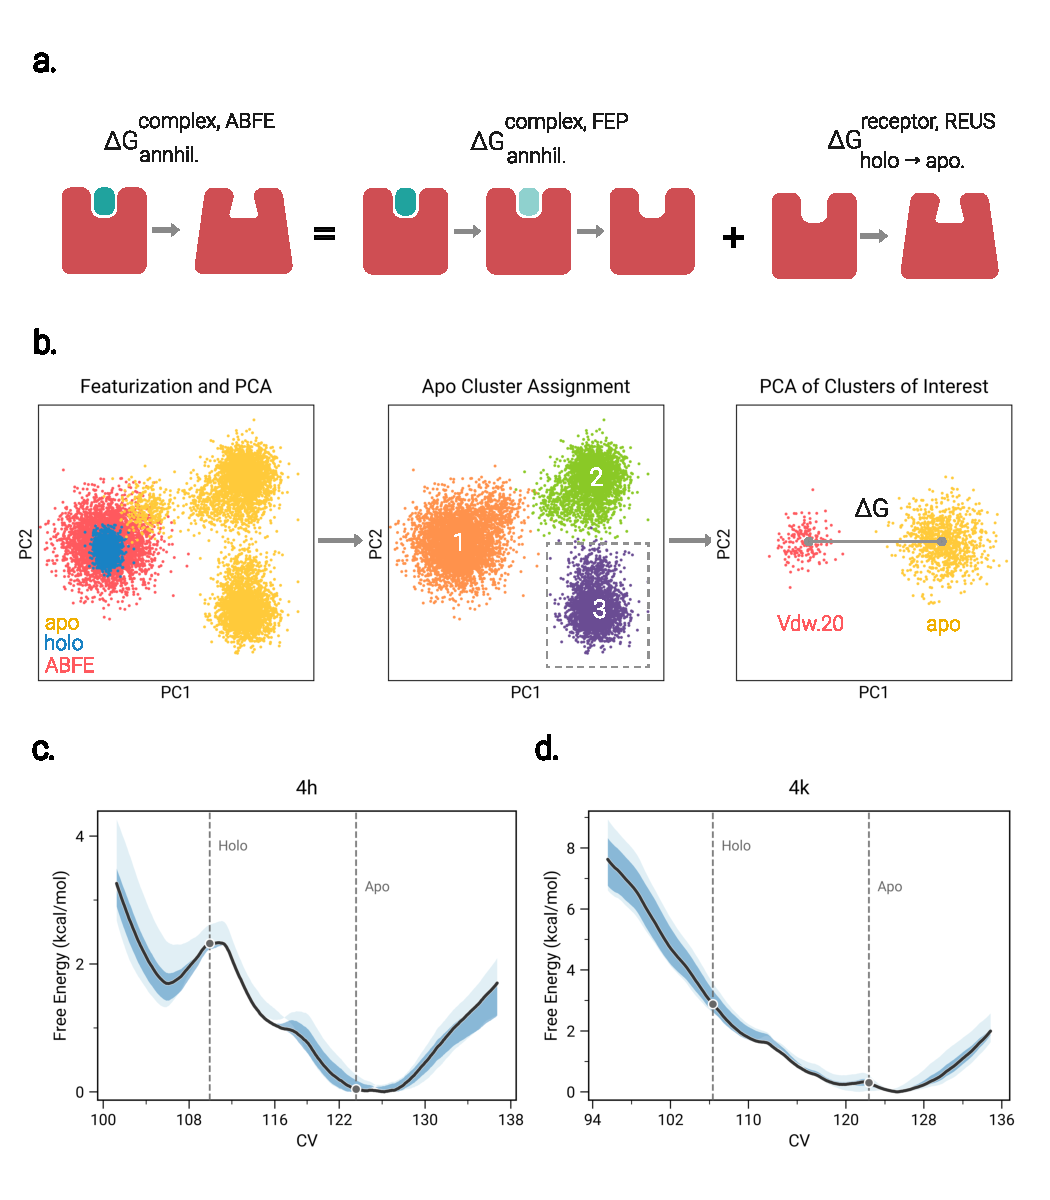
\includegraphics[width=\textwidth,height=0.66\textheight,keepaspectratio]{chapters/Ch5-Apo-state-conformational-changes/figures/apo_state_correction/paper_figure_7.pdf}
  \caption[REUS framework for correcting apo-state representation.]{Correction of systematic overestimation in the Deflorian A$_{2A}$ receptor dataset. (a) Thermodynamic cycle incorporating receptor relaxation from holo-like to apo-like states as an additional free-energy contribution. (b) Construction of the collective variable: pairwise C$\alpha$ distances describe the binding pocket; PCA and clustering identify apo-like states; selected apo and final ABFE-window structures then define a refined one-dimensional PCA coordinate for replica-exchange umbrella sampling (REUS). Example free-energy surfaces show (c) distinct apo-like and holo-like wells for compound 4h and (d) no clear separating barrier for compound 4k.}
  \label{fig:apo-state-reus-framework}
  \caption*{Reproduced from Figure 7 of Anand et al.\cite{anand2026improving} under CC BY 4.0.}
\end{figure}

The clustering, selected apo/endpoint projections, and compound-specific REUS
profiles are shown in Figures~\ref{fig:si-pca-clusters},
\ref{fig:si-pca-endpoint-cv}, and~\ref{fig:si-reus-free-energy-surfaces}.

\subsection{Using a PC1 of the C alphas as CV for 1 ligand}

\lipsum[1][1-3]

\subsection{Using binding pocket CV for 1 ligand}

\lipsum[1][1-3]

\subsection{Extra polating to other ligands}

\lipsum[1][1-3]

\begin{figure}[htbp]
  \centering
  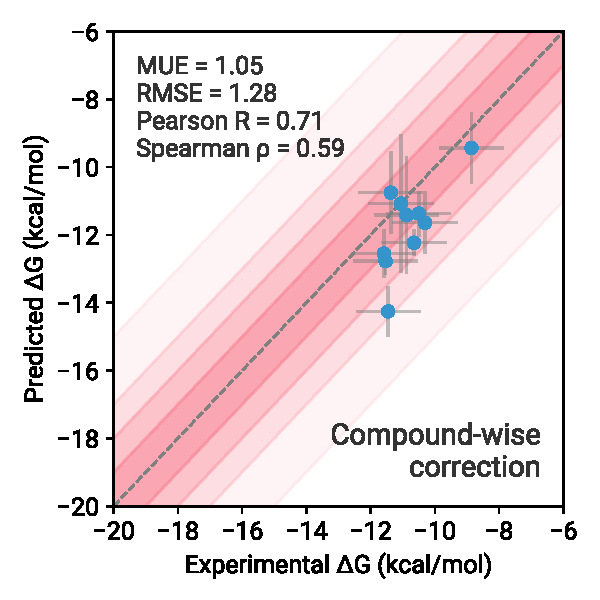
\includegraphics[width=0.78\textwidth,height=0.52\textheight,keepaspectratio]{chapters/Ch5-Apo-state-conformational-changes/figures/compound_correction/paper_figure_8.pdf}
  \caption[Compound-specific receptor relaxation corrections.]{Improvement in ABFE binding-affinity predictions for the Deflorian A$_{2A}$ receptor dataset following compound-specific receptor relaxation corrections.}
  \label{fig:compound-specific-apo-correction}
  \caption*{Reproduced from Figure 8 of Anand et al.\cite{anand2026improving} under CC BY 4.0.}
\end{figure}

\subsection{Correcting with a common apo state correction}

\lipsum[1][1-3]

\begin{figure}[htbp]
  \centering
  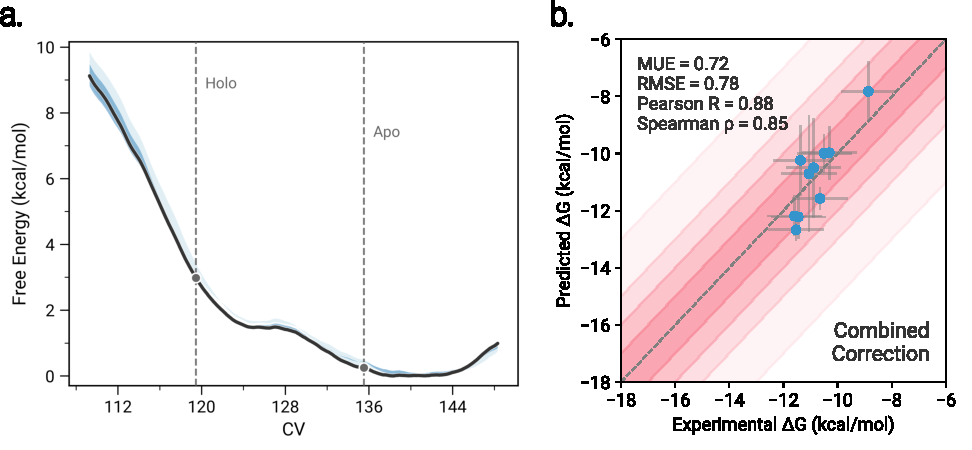
\includegraphics[width=\textwidth]{chapters/Ch5-Apo-state-conformational-changes/figures/combined_correction/paper_figure_9.pdf}
  \caption[A common receptor relaxation correction for the combined dataset.]{Conformational free-energy contributions to ABFE calculations. (a) Free-energy surface from REUS using the combined dataset, describing relaxation from holo-like structures in the noninteracting ABFE window to an apo-like state identified from long apo simulations. (b) Improved binding-affinity predictions after applying a single receptor relaxation correction to the combined dataset.}
  \label{fig:common-apo-correction}
  \caption*{Reproduced from Figure 9 of Anand et al.\cite{anand2026improving} under CC BY 4.0.}
\end{figure}

\section{Conclusions}
% TODO: Add content here.
\lipsum[1][1-3]
